\chapter{系统实现}
\label{cha:implementation}

\section{系统实现与运行环境}
\label{sec:env}

本系统的实现采用的编程语言是Python,具体来说是Python3,因为Python很适合编写服务器以及其语法比较简单,
也有丰富的库可以使用,其中就包括三个互联网设备搜索已经的API,用来处理API返回的json十分简单。服务器使用的框架是Flask,
因为其比较轻量级,功能也比较齐全,也提供了模板引擎,可以大大简化工作,所以选择了Flask。

系统的开发环境是MacOS,不过可以在安装了相应依赖的任何操作系统上运行。目前本系统在一台Linux服务器上运行。

\section{模块划分}
\label{sec:modules}

依据第三章的介绍,本系统共划分为6个模块,分别是网站信息抓取模块,具体完成主机信息的抓取;CVE信息抓取模块,完成CVE信息的抓取;
数据库操作模块,完成对数据库的读写;推送模块,在完成了威胁情报的分析之后,由该模块进行用户通知的推送;中央控制模块,控制整个系统的运行,
包括控制信息抓取的开始与结束,控制信息的存储于读取,威胁情报的分析和最终的推送也在这个模块完成;还有一个网站的部分,仅依赖于系统中的数据库。

在接下来的6节里讲分别介绍这6个模块。

\section{主机信息抓取模块}
\label{sec:hosts-module}

因为主机信息的工具是互联网搜索引擎的API,而这些API各不相同,肯定要单独写函数,但是,
对于很多的关键词抓取,它们的行为又是一样的,也即遍历所有的关键词,对关键词进行检索,而当关键词比较多的时候,
对关键词列表的增删操作也是一样的。因此,为了扩展性,将来可以添加更多的互联网搜索引擎API进入这个系统,
系统首先定义了一个信息抓取的基类Aggregator,这个基类中一个成员变量表示所有的需要检索的关键词列表,这个列表的每一个成员都是一个Query变量,
这个变量将在下文中介绍。在Aggregator类中,实现了对这个Query的列表的操作,如设置列表内容,增加或者删除一个Query,等等。然后,
也实现了对全部的Query进行检索的方法,也即遍历列表依次检索并存入一个格式化的返回列表中。而对于每一个Query如何进行检索是依API不同而异的,
因此对一个Query进行信息抓取的函数是一个抽象方法,由继承它的各个具体的Aggregator来实现。

在使用具体的信息抓取类进行抓取操作时,首先实例化一个Aggregator对象,然后设定它的queries列表,调用fetch\_all即可实现抓取操作。

上文中提到的Query类,之所以不直接用一个字符串来表示一个检索的目标,是因为一个检索很可能不仅是一个字符串那么简单,
它可能有一些其他的限制条件,比如排除其中的一些主机等,而每个API的语法都是不同的,如果仅把这些内容用字符串来表示,
可能对于每个API来说传递给它们的字符串就会不同,这会影响可扩展性。相反,如果在初始化设定检索目标的时候,就把这些信息存入对象,
而具体的各个Aggregator来实现对这些信息的读取和生成查询API时的语句,就能解决这个问题。目前Query类只有两个成员变量,
一个是表示检索对象的query,一个是表示对象的类型的query\_type,如表示域名的hostname、表示IP地址段的net和表示IP地址的ip。
虽然可以由系统自动判断类别,但是目前的实现是在配置文件中由用户指定目标具体属于哪一类。

\begin{figure}[H]
    \centering
    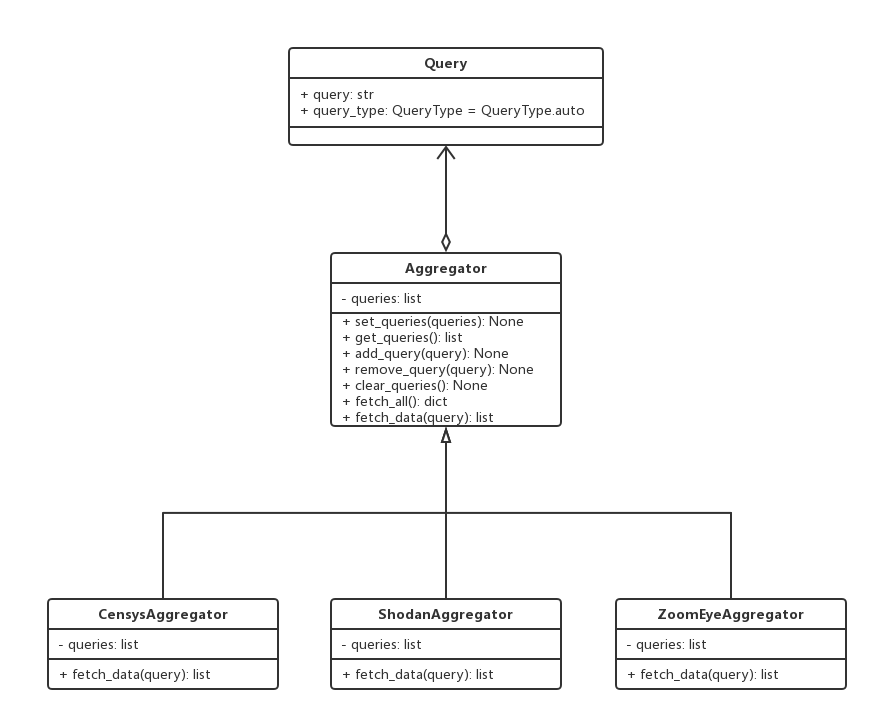
\includegraphics[scale=0.35]{hosts-aggregation-class.png}
    \caption{主机信息抓取模块类图}
    \label{fig:comparation}
\end{figure}

具体的Aggregator目前有3个,分别是CensysAggregator,ShodanAggregator和ZoomEyeAggregator。这三个类都继承了Aggregator类,
实现了其中的抽象方法。图4.1是该模块的类图。从图中可以看出,三个具体的Aggregator类和Aggregator基类是继承院系,
而Aggregator和Query是聚合关系。

接下来依次介绍每一个API的信息抓取的类。

首先是CensysAggregator。Censys的API的参数中有一个是page,表示需要结果第几页,一页有100个结果,因此第一页就是第1至100个结果,
第二页就是第101至第200个结果,以此类推。因此在CensysAggregator内部又实现了一个方法fetch\_page,可以抓取一页最多100条结果的信息。
而在返回的结果中,有一个字段“metadata”会记录这些结果的元数据,在“metadata”字段中的“pages”字段就能知道这个关键词的搜索结果会有多少页。
所以,首先获得第一页的数据,看到有多少页之后循环获得后面几页的数据后再合并成一个新的列表,再给每个结果加上一个“source”字段赋值为“Censys”即可。

然后是ShodanAggregator。类似于Censys,Shodan的结果也是分页的,但是由于Shodan的API /search的结果只返回部分数据,
需要对每一个结果主机再次进行查询,因此,对每一个主机仅记录其IP地址,然后再对每一页的IP地址列表进行合并,删除重复的。
接着用另一个成员方法get\_info\_by\_ip获得其中每一台主机的详细信息,最后加入“source”字段赋值为“Shodan”。其中值得注意的一点是,
/host的API是有失败的可能的,因此在实现的时候设置了一个尝试次数,用try语句尝试几次,如果都失败了才最终返回一个只含IP地址的主机信息。

最后是ZoomEyeAggregator。ZoomEye的做法和Censys基本一样,也是先获得一页的内容然后再判断有多少页,
不过稍微不同的是ZoomEye没有直接提供页数的字段,而是总的可用的条目数“available”,需要自己计算页数。
在ZoomEyeAggregator中还实现了一个方法get\_latest,这个方法是在进行融合的时候使用。因为ZoomEye提供数据里面有重复的,
因此在融合的时候需要把相同主机的数据里面选出更新时间最新的数据,也即“timestamp”字段最大的数据。



